\documentclass[tikz,border=5mm]{standalone}
\usetikzlibrary{calc,angles,quotes,intersections,through,positioning,3d,arrows.meta}
\begin{document}
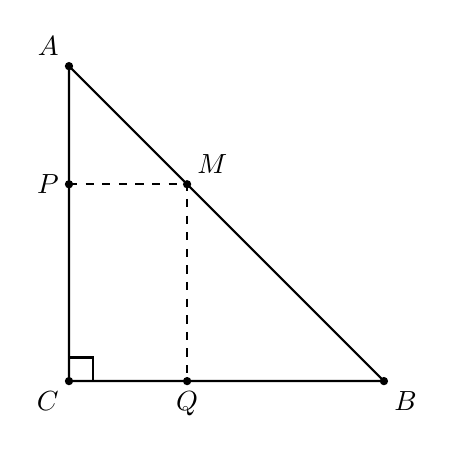
\begin{tikzpicture}[thick]
\coordinate (C) at (0,0);\coordinate (A) at (0,4);\coordinate (B) at (4,0);
\coordinate (P) at (0,2.5);\coordinate (Q) at (1.5,0);\coordinate (M) at (1.5,2.5);
\draw (A)--(B)--(C)--cycle;\draw[dashed] (P)--(M)--(Q);
\pic[draw,angle radius=0.3cm]{right angle=A--C--B};
\foreach \p in {A,B,C,P,Q,M}{\fill (\p) circle (1.5pt);}
\node[above left] at (A) {$A$};\node[below left] at (C) {$C$};\node[below right] at (B) {$B$};\node[left] at (P) {$P$};\node[below] at (Q) {$Q$};\node[above right] at (M) {$M$};
\end{tikzpicture}\end{document}